\documentclass[tikz,border=3pt]{standalone}
\usetikzlibrary{arrows.meta}
\begin{document}
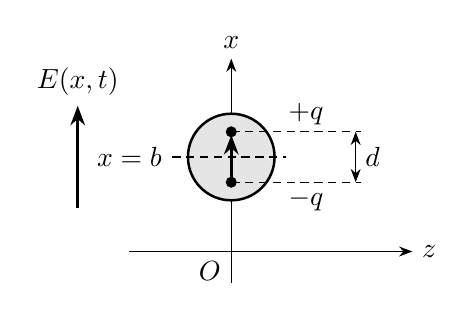
\begin{tikzpicture}[scale=1.0,>=Stealth,line width=0.9pt]
  % 座標軸
  \draw[line width=0.4pt,->] (-1.3,0) -- (2.3,0) node[right] {$z$};
  \draw[line width=0.4pt,->] (0,-0.4) -- (0,2.45) node[above] {$x$};
  \node[below left] at (0,0) {$O$};

  % 誘電体球（中心 x = b = 1.2）
  \draw[fill=black!10] (0,1.2) circle (0.55);
  \draw[line width=0.4pt,densely dashed] (-0.75,1.2) -- (0.70,1.2);
  \node[left] at (-0.75,1.2) {$x = b$};

  % 微小電気双極子 (+q at b+d/2, -q at b-d/2)
  \fill (0,1.52) circle (2.0pt);
  \fill (0,0.88) circle (2.0pt);
  \draw[->] (0,0.88) -- (0,1.48);

  % +q, -q と間隔 d の表示（円周と重ならない位置に配置）
  \draw[line width=0.4pt,densely dashed] (0,1.52) -- (1.65,1.52);
  \draw[line width=0.4pt,densely dashed] (0,0.88) -- (1.65,0.88);
  \node[above,inner sep=1.5pt] at (0.95,1.54) {$+q$};
  \node[below,inner sep=1.5pt] at (0.95,0.86) {$-q$};
  \draw[line width=0.4pt,<->] (1.58,0.88) -- (1.58,1.52) node[midway,right] {$d$};

  % 入射電場の向き（左側に十分離して配置）
  \draw[->] (-1.95,0.55) -- (-1.95,1.85) node[above] {$E(x,t)$};
\end{tikzpicture}
\end{document}
